\documentclass[10pt,aspectratio=169]{beamer}

% =====================================================
% PAQUETES
% =====================================================

\usepackage[utf8]{inputenc}
\usepackage[T1]{fontenc}
\usepackage[spanish]{babel}

\usepackage{amsmath}
\usepackage{amsfonts}
\usepackage{amssymb}

\usepackage{graphicx}
\usepackage{tikz}
\usepackage{booktabs}
\usepackage{array}
\usepackage{ragged2e}

% =====================================================
% CONFIGURACIÓN GENERAL
% =====================================================

\usetheme{default}

\setbeamertemplate{navigation symbols}{}
\setbeamertemplate{headline}{}
\setbeamertemplate{footline}{}

% =====================================================
% COLORES
% =====================================================

\definecolor{unemiAzul}{RGB}{20,40,90}
\definecolor{unemiNaranja}{RGB}{255,102,0}

% =====================================================
% TIPOGRAFÍA
% =====================================================

\setbeamerfont{frametitle}{size=\Large,series=\bfseries}
\setbeamercolor{frametitle}{fg=unemiAzul}

% =====================================================
% FONDO GENERAL
% =====================================================

\setbeamertemplate{background}{
	\begin{tikzpicture}[remember picture,overlay]
		\node[inner sep=0pt] at (current page.center){
			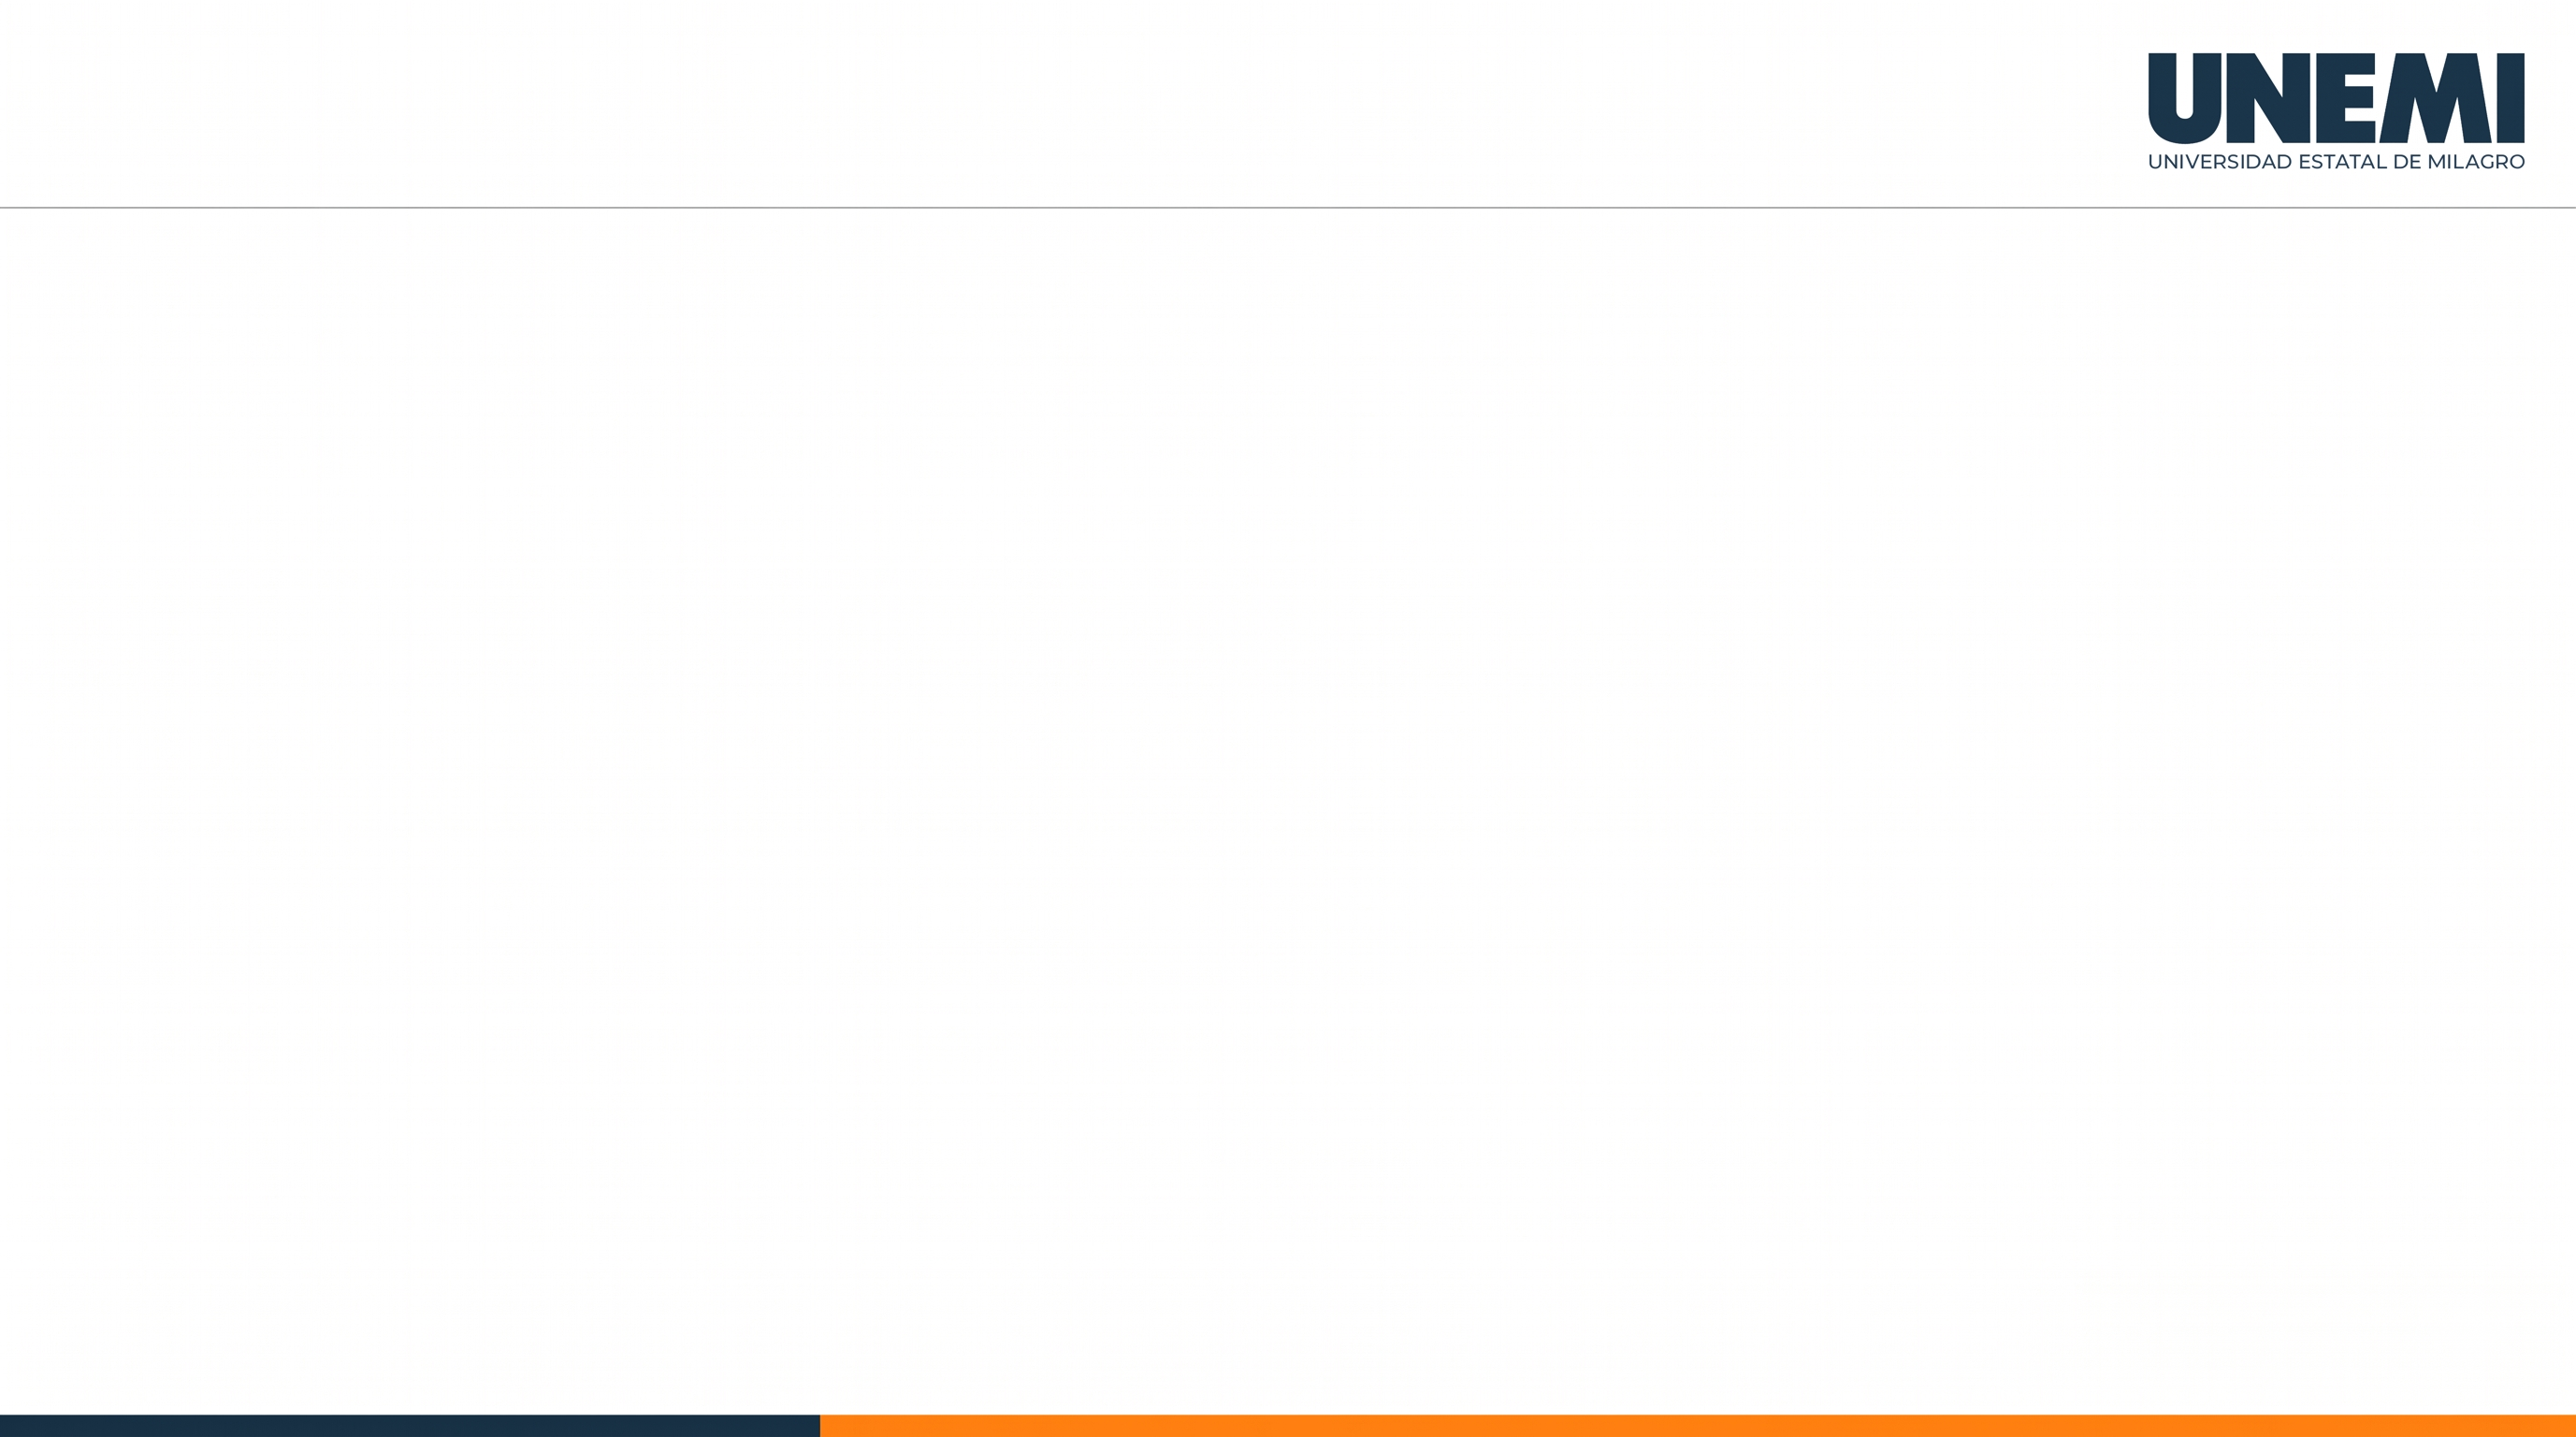
\includegraphics[width=\paperwidth,height=\paperheight]{portadaUNEMI2}
		};
	\end{tikzpicture}
}

% =====================================================
% INICIO DEL DOCUMENTO
% =====================================================

\begin{document}
	
	% =====================================================
	% PORTADA
	% =====================================================
	
	{
		\setbeamertemplate{background}{
			
\includegraphics[width=\paperwidth,height=\paperheight]{portadaUNEMI}
		}
		
		\begin{frame}[plain]
			
			\begin{tikzpicture}[remember picture,overlay]
				
				\node[
				fill=unemiAzul,
				fill opacity=0.85,
				text opacity=1,
				rounded corners,
				inner sep=20pt
				]
				at (current page.center)
				{
					\begin{minipage}{0.75\textwidth}
						
						\centering
						
						{\Huge \textbf{\textcolor{white}{
									Aritmética del Computador,
									Fundamentos de TI y Hardware
						}}}
						
						\vspace{0.5cm}
						
						{\Large \textcolor{white}{
								Investigación académica utilizando el método Feynman
						}}
						
						\vspace{1cm}
						
						{\small \textcolor{white}{Estudiante}}
						
						\vspace{0.2cm}
						
						{\Large \textcolor{unemiNaranja}{
								Angel Fernando Calero Maldonado
						}}
						
						\vspace{0.5cm}
						
						{\small \textcolor{white}{
								Universidad Estatal de Milagro
						}}
						
					\end{minipage}
				};
				
			\end{tikzpicture}
			
		\end{frame}
		
	}
	
	% =====================================================
	% ÍNDICE
	% =====================================================
	
	\begin{frame}{Índice de la Presentación}
		
		\small
		
		\begin{block}{Tema 3: Aritmética del computador}
			\begin{itemize}
				\item Subtema 1: Presentación
				\item Subtema 2: Aritmética del computador
				\item Subtema 3: Unidades de medida
				\item Subtema 4: Lógica
			\end{itemize}
		\end{block}
		
		\begin{block}{Tema 4: Fundamentos de TI}
			\begin{itemize}
				\item Subtema 1: Presentación
				\item Subtema 2: Elementos de un computador
				\item Subtema 3: Representación de la información
				\item Subtema 4: La computadora en la actualidad
			\end{itemize}
		\end{block}
		
		\begin{block}{Tema 5: Fundamentos de hardware}
			\begin{itemize}
				\item Subtema 1: Presentación
				\item Subtema 2: Estructura y organización de un computador
				\item Subtema 3: Funcionamiento interno del computador
				\item Subtema 4: Memoria y periféricos
			\end{itemize}
		\end{block}
		
	\end{frame}
	
	% =====================================================
	% MÉTODO FEYNMAN
	% =====================================================
	
	\begin{frame}{Método Feynman aplicado}
		
		\begin{block}{Idea principal}
			El método Feynman consiste en aprender un tema explicándolo con palabras simples, como si se enseñara a una persona sin conocimientos técnicos.
		\end{block}
		
		\begin{itemize}
			\item Explicar conceptos complejos de forma sencilla.
			\item Utilizar ejemplos cotidianos.
			\item Detectar vacíos de comprensión.
			\item Reestructurar las ideas con claridad.
		\end{itemize}
		
		\vspace{0.3cm}
		
		\textbf{Objetivo:}
		Comprender cómo funcionan las computadoras desde la lógica matemática hasta su estructura física.
		
	\end{frame}
	
	% =====================================================
	% TEMA 3
	% =====================================================
	
	\begin{frame}{Tema 3: Aritmética del computador}
		
		\begin{block}{Explicación sencilla}
			La computadora realiza cálculos utilizando únicamente dos estados eléctricos representados mediante 0 y 1.
		\end{block}
		
		\begin{itemize}
			\item Todo dato se convierte en código binario.
			\item Las operaciones matemáticas son ejecutadas por circuitos electrónicos.
			\item La Unidad Aritmético-Lógica procesa cálculos y comparaciones.
			\item El sistema binario es la base de toda computación digital.
		\end{itemize}
		
	\end{frame}
	
	% =====================================================
	% SUBTEMA 3.1
	% =====================================================
	
	\begin{frame}{Subtema 3.1: Presentación}
		
		\begin{block}{Analogía Feynman}
			Una computadora es como una calculadora extremadamente rápida que sigue instrucciones exactas millones de veces por segundo.
		\end{block}
		
		\begin{itemize}
			\item La computadora no piensa como un humano.
			\item Sigue reglas matemáticas precisas.
			\item Los circuitos internos ejecutan operaciones eléctricas.
			\item Todo el procesamiento ocurre mediante señales binarias.
		\end{itemize}
		
	\end{frame}
	
	% =====================================================
	% SUBTEMA 3.2
	% =====================================================
	
	\begin{frame}{Subtema 3.2: Aritmética del computador}
		
		\small
		
		\begin{block}{Sistema binario}
			El sistema binario utiliza únicamente los símbolos 0 y 1.
		\end{block}
		
		\[
		1011_2 =
		1(2^3)+0(2^2)+1(2^1)+1(2^0)=11_{10}
		\]
		
		\begin{itemize}
			\item Los bits representan estados eléctricos.
			\item Las operaciones binarias permiten realizar cálculos.
			\item La ALU ejecuta sumas, restas y operaciones lógicas.
			\item Los computadores modernos utilizan millones de transistores para procesar datos.
		\end{itemize}
		
	\end{frame}
	
	% =====================================================
	% COMPLEMENTO A DOS
	% =====================================================
	
	\begin{frame}{Complemento a dos}
		
		\begin{block}{Explicación sencilla}
			El complemento a dos permite representar números negativos utilizando el mismo hardware de suma.
		\end{block}
		
		\begin{itemize}
			\item Se invierten los bits.
			\item Luego se suma 1.
			\item Facilita operaciones matemáticas internas.
		\end{itemize}
		
		\vspace{0.3cm}
		
		\begin{block}{Ejemplo}
			\[
			5 = 00000101
			\]
			
			Invertir bits:
			
			\[
			11111010
			\]
			
			Sumar 1:
			
			\[
			11111011 = -5
			\]
		\end{block}
		
	\end{frame}
	
	% =====================================================
	% PUNTO FLOTANTE
	% =====================================================
	
	\begin{frame}{Representación en punto flotante}
		
		\small
		
		\begin{block}{Explicación sencilla}
			El punto flotante permite representar números decimales utilizando una estructura similar a la notación científica.
		\end{block}
		
		\begin{itemize}
			\item Divide el número en signo, exponente y mantisa.
			\item Permite manejar números muy grandes o pequeños.
			\item Utiliza el estándar IEEE 754.
			\item Algunos decimales no pueden representarse exactamente.
		\end{itemize}
		
		\begin{block}{Ejemplo cotidiano}
			Por esta razón, algunos lenguajes muestran resultados como:
			
			\[
			0.1 + 0.2 \neq 0.3
			\]
		\end{block}
		
	\end{frame}
	
	% =====================================================
	% SUBTEMA 3.3
	% =====================================================
	
	\begin{frame}{Subtema 3.3: Unidades de medida}
		
		\small
		
		\begin{block}{Bit y byte}
			El bit es la unidad mínima de información y un byte equivale a 8 bits.
		\end{block}
		
		\begin{center}
			
			\begin{tabular}{>{\bfseries}c c}
				
				\toprule
				
				Unidad & Equivalencia \\
				
				\midrule
				
				1 bit & 0 o 1 \\
				
				1 byte & 8 bits \\
				
				1 KB & 1024 bytes \\
				
				1 MB & 1024 KB \\
				
				1 GB & 1024 MB \\
				
				1 TB & 1024 GB \\
				
				\bottomrule
				
			\end{tabular}
			
		\end{center}
		
	\end{frame}
	
	% =====================================================
	% SUBTEMA 3.4
	% =====================================================
	
	\begin{frame}{Subtema 3.4: Lógica}
		
		\begin{block}{Explicación sencilla}
			La lógica digital permite que el computador tome decisiones mediante valores verdaderos o falsos.
		\end{block}
		
		\begin{itemize}
			\item AND: ambas entradas deben ser 1.
			\item OR: al menos una entrada debe ser 1.
			\item NOT: invierte el valor.
			\item XOR: detecta diferencias entre entradas.
		\end{itemize}
		
		\begin{block}{Analogía}
			Una puerta AND funciona como una puerta con dos llaves: ambas deben activarse para abrirse.
		\end{block}
		
	\end{frame}
	
	% =====================================================
	% TEMA 4
	% =====================================================
	
	\begin{frame}{Tema 4: Fundamentos de TI}
		
		\begin{block}{Explicación sencilla}
			Las Tecnologías de la Información integran hardware, software, redes y datos para procesar información útil.
		\end{block}
		
		\begin{itemize}
			\item Permiten almacenar grandes cantidades de información.
			\item Facilitan la comunicación global.
			\item Automatizan procesos empresariales y académicos.
			\item Conectan personas y sistemas digitales.
		\end{itemize}
		
	\end{frame}
	
	% =====================================================
	% SUBTEMA 4.1
	% =====================================================
	
	\begin{frame}{Subtema 4.1: Presentación}
		
		\begin{block}{Analogía Feynman}
			Las TI funcionan como el sistema nervioso de una organización.
		\end{block}
		
		\begin{itemize}
			\item El hardware actúa como el cuerpo físico.
			\item El software contiene las instrucciones.
			\item Las redes permiten la comunicación.
			\item Los datos representan el conocimiento.
		\end{itemize}
		
	\end{frame}
	
	% =====================================================
	% SUBTEMA 4.2
	% =====================================================
	
	\begin{frame}{Subtema 4.2: Elementos de un computador}
		
		\small
		
		\begin{center}
			
			\begin{tabular}{>{\bfseries}p{3cm} p{8cm}}
				
				\toprule
				
				Elemento & Función \\
				
				\midrule
				
				CPU & Ejecuta instrucciones y coordina operaciones. \\
				
				RAM & Guarda temporalmente datos y programas activos. \\
				
				Almacenamiento & Conserva información permanentemente. \\
				
				Entrada & Permite ingresar información al sistema. \\
				
				Salida & Presenta resultados al usuario. \\
				
				Red & Conecta dispositivos y sistemas. \\
				
				\bottomrule
				
			\end{tabular}
			
		\end{center}
		
	\end{frame}
	
	% =====================================================
	% SUBTEMA 4.3
	% =====================================================
	
	\begin{frame}{Subtema 4.3: Representación de la información}
		
		\begin{block}{Idea principal}
			Toda información digital se representa mediante secuencias binarias.
		\end{block}
		
		\begin{itemize}
			\item Texto: ASCII y Unicode.
			\item Imágenes: píxeles y colores.
			\item Audio: muestras digitales.
			\item Video: imágenes sucesivas y sonido sincronizado.
		\end{itemize}
		
		\begin{block}{Explicación Feynman}
			Para el computador, una canción, una fotografía y un documento son únicamente diferentes formas de organizar bits.
		\end{block}
		
	\end{frame}
	
	% =====================================================
	% SUBTEMA 4.4
	% =====================================================
	
	\begin{frame}{Subtema 4.4: La computadora en la actualidad}
		
		\small
		
		\begin{block}{Transformación digital}
			Las computadoras modernas están presentes en prácticamente todos los ámbitos de la sociedad.
		\end{block}
		
		\begin{itemize}
			\item Inteligencia artificial.
			\item Computación en la nube.
			\item Internet de las cosas.
			\item Ciberseguridad.
			\item Automatización industrial.
		\end{itemize}
		
	\end{frame}
	
	% =====================================================
	% TEMA 5
	% =====================================================
	
	\begin{frame}{Tema 5: Fundamentos de hardware}
		
		\begin{block}{Explicación sencilla}
			El hardware corresponde a todos los componentes físicos que permiten el funcionamiento del computador.
		\end{block}
		
		\begin{itemize}
			\item Procesador.
			\item Memoria.
			\item Placa madre.
			\item Discos de almacenamiento.
			\item Periféricos.
		\end{itemize}
		
	\end{frame}
	
	% =====================================================
	% SUBTEMA 5.1
	% =====================================================
	
	\begin{frame}{Subtema 5.1: Presentación}
		
		\begin{block}{Analogía Feynman}
			El hardware funciona como una fábrica donde cada componente cumple una tarea específica.
		\end{block}
		
		\begin{itemize}
			\item La CPU coordina operaciones.
			\item La memoria entrega datos rápidamente.
			\item El almacenamiento conserva información.
			\item Los buses transportan datos internos.
		\end{itemize}
		
	\end{frame}
	
	% =====================================================
	% SUBTEMA 5.2
	% =====================================================
	
	\begin{frame}{Subtema 5.2: Estructura y organización de un computador}
		
		\small
		
		\begin{block}{Arquitectura de Von Neumann}
			La computadora almacena instrucciones y datos en memoria para ser ejecutados por la CPU.
		\end{block}
		
		\begin{itemize}
			\item Unidad de control.
			\item Unidad aritmético-lógica.
			\item Memoria principal.
			\item Entrada y salida.
		\end{itemize}
		
		\begin{block}{Idea clave}
			La computadora repite constantemente el ciclo:
			buscar, decodificar y ejecutar instrucciones.
		\end{block}
		
	\end{frame}
	
	% =====================================================
	% SUBTEMA 5.3
	% =====================================================
	
	\begin{frame}{Subtema 5.3: Funcionamiento interno del computador}
		
		\small
		
		\begin{block}{Ciclo de instrucción}
			La CPU sigue una secuencia repetitiva para ejecutar programas.
		\end{block}
		
		\begin{enumerate}
			\item Buscar instrucciones.
			\item Decodificar instrucciones.
			\item Ejecutar operaciones.
			\item Guardar resultados.
		\end{enumerate}
		
		\begin{block}{Explicación sencilla}
			Un programa funciona como una receta que la CPU sigue paso a paso.
		\end{block}
		
	\end{frame}
	
	% =====================================================
	% REGISTROS Y BUSES
	% =====================================================
	
	\begin{frame}{Registros, buses y reloj}
		
		\small
		
		\begin{itemize}
			\item Registros: memorias internas extremadamente rápidas.
			\item Buses: canales por donde viajan los datos.
			\item Reloj: sincroniza operaciones del procesador.
			\item Caché: memoria rápida para datos frecuentes.
		\end{itemize}
		
		\begin{block}{Analogía}
			Los registros son notas rápidas en la mano; el disco duro es una biblioteca más lenta pero permanente.
		\end{block}
		
	\end{frame}
	
	% =====================================================
	% SUBTEMA 5.4
	% =====================================================
	
	\begin{frame}{Subtema 5.4: Memoria y periféricos}
		
		\small
		
		\begin{center}
			
			\begin{tabular}{>{\bfseries}p{3cm} p{8cm}}
				
				\toprule
				
				Componente & Función \\
				
				\midrule
				
				RAM & Memoria temporal y volátil. \\
				
				ROM & Instrucciones básicas de arranque. \\
				
				SSD/HDD & Almacenamiento permanente. \\
				
				Entrada & Capturan datos del usuario. \\
				
				Salida & Muestran información procesada. \\
				
				Mixtos & Envían y reciben información. \\
				
				\bottomrule
				
			\end{tabular}
			
		\end{center}
		
	\end{frame}
	
	% =====================================================
	% COMPARACIÓN GENERAL
	% =====================================================
	
	\begin{frame}{Comparación general de los tres temas}
		
		\small
		
		\begin{center}
			
			\begin{tabular}{>{\bfseries}p{3cm} p{8cm}}
				
				\toprule
				
				Tema & Pregunta principal \\
				
				\midrule
				
				Aritmética del computador & ¿Cómo calcula una computadora? \\
				
				Fundamentos de TI & ¿Cómo se usa la tecnología para procesar información? \\
				
				Fundamentos de hardware & ¿Qué componentes físicos permiten el funcionamiento? \\
				
				\bottomrule
				
			\end{tabular}
			
		\end{center}
		
		\vspace{0.4cm}
		
		\begin{block}{Síntesis}
			El hardware es el cuerpo físico, la aritmética binaria es el lenguaje interno y las TI representan el uso organizado de toda la tecnología.
		\end{block}
		
	\end{frame}
	
	% =====================================================
	% CONCLUSIONES
	% =====================================================
	
	\begin{frame}{Conclusiones}
		
		\begin{itemize}
			\item La aritmética del computador permite comprender cómo las máquinas procesan datos mediante lógica binaria.
			\item Las Tecnologías de la Información integran hardware, software y redes para resolver problemas reales.
			\item El hardware constituye la base física del procesamiento digital.
			\item Comprender estos conceptos permite utilizar la tecnología de manera crítica y técnica.
		\end{itemize}
		
	\end{frame}
	
	% =====================================================
	% REFERENCIAS
	% =====================================================
	
	\begin{frame}{Fuentes académicas consultadas}
		
		\tiny
		
		\begin{itemize}
			
			\item Patterson, D. A., \& Hennessy, J. L. (2021). \textit{Computer Organization and Design}. Morgan Kaufmann.
			
			\item Stallings, W. (2022). \textit{Computer Organization and Architecture}. Pearson.
			
			\item Bryant, R. E., \& O'Hallaron, D. R. (2016). \textit{Computer Systems: A Programmer's Perspective}. Pearson.
			
			\item Tanenbaum, A. S. (2013). \textit{Structured Computer Organization}. Pearson.
			
			\item Mano, M. M., \& Ciletti, M. D. (2017). \textit{Digital Design}. Pearson.
			
			\item IEEE Computer Society. (2019). \textit{IEEE Standard 754-2019}.
			
			\item MIT OpenCourseWare. \textit{Computation Structures}.
			
			\item Harvard University. \textit{CS50 Introduction to Computer Science}.
			
			\item NIST. (2008). \textit{Guide for the Use of the International System of Units}.
			
		\end{itemize}
		
	\end{frame}
	
	% =====================================================
	% DIAPOSITIVA FINAL
	% =====================================================
	
	{
		\setbeamertemplate{background}{
			
\includegraphics[width=\paperwidth,height=\paperheight]{portadaUNEMI}
		}
		
		\begin{frame}[plain]
			
			\begin{tikzpicture}[remember picture,overlay]
				
				\node[
				fill=unemiAzul,
				fill opacity=0.85,
				text opacity=1,
				rounded corners,
				inner sep=20pt
				]
				at (current page.center)
				{
					\begin{minipage}{0.8\textwidth}
						
						\centering
						
						{\Huge \textbf{\textcolor{white}{Gracias}}}
						
						\vspace{0.5cm}
						
						{\Large \textcolor{white}{Preguntas y comentarios}}
						
					\end{minipage}
				};
				
			\end{tikzpicture}
			
		\end{frame}
		
	}
	
	% =====================================================
	% FIN DEL DOCUMENTO
	% =====================================================
	
\end{document}